\documentclass[12pt]{APA7}

% Use Times New Roman
\setmainfont{Times New Roman}
% Indent the first line of a new paragraph by 0.5 inches
\setlength{\parindent}{0.5in}


%%
% Author: Rui Sun
% Mailto: r.sun.22@ucl.ac.uk
% Update Date: 12 Sep 2024
% Replace with your own information
% Good luck with your thesis (‐^▽^‐)
%%

% Ignore this file in word count
%TC:ignore
\titlefirst{First Line of Your Title}
\titlesecond{Second Line of Your Title}
\titlethird{Third Line of Your Title}

\program{MSc Psychology}

\supervisor{Prof. Anna and Dr Bob}

\wordcount{12345}

\candidatenumber{ABCD1}
%TC:endignore

\begin{document}

% Cover of your essay
\makecover

\pagenumbering{arabic}

% Include Abstract
\section{Abstract}

write your research background, research gap, main findings, and implication.


% ToC
{\setlength{\baselineskip}{0.8\baselineskip} % line space
\setcounter{tocdepth}{2} % Set depth of ToC
\tableofcontents}

% new page
\clearpage

% LoF
\listoffigures

% Include Main Body
\section{Introduction}

briefly introduction

\subsection{Section 1}

review some previous studies

You could use "parencite" or "textcite" function to cite artciles. Following are two examples:

\parencite{hauser_social_2019}

\textcite{Efferson2024super}

\subsection{Section 2}

review some previous studies

\subsection{Present Study}

introduce your research questions, hypotheses, research paradigms and predictions
\section{Study 1}

\subsection{Methods}

\subsubsection{Participants}

sample size, demographics, participant fees, informed consent

\subsubsection{Design \& Materials}

procedures, IVs, DVs, etc.

\subsection{Results}

\begin{figure}[h]
    \centering
    
    \begin{subfigure}{0.48\linewidth}
        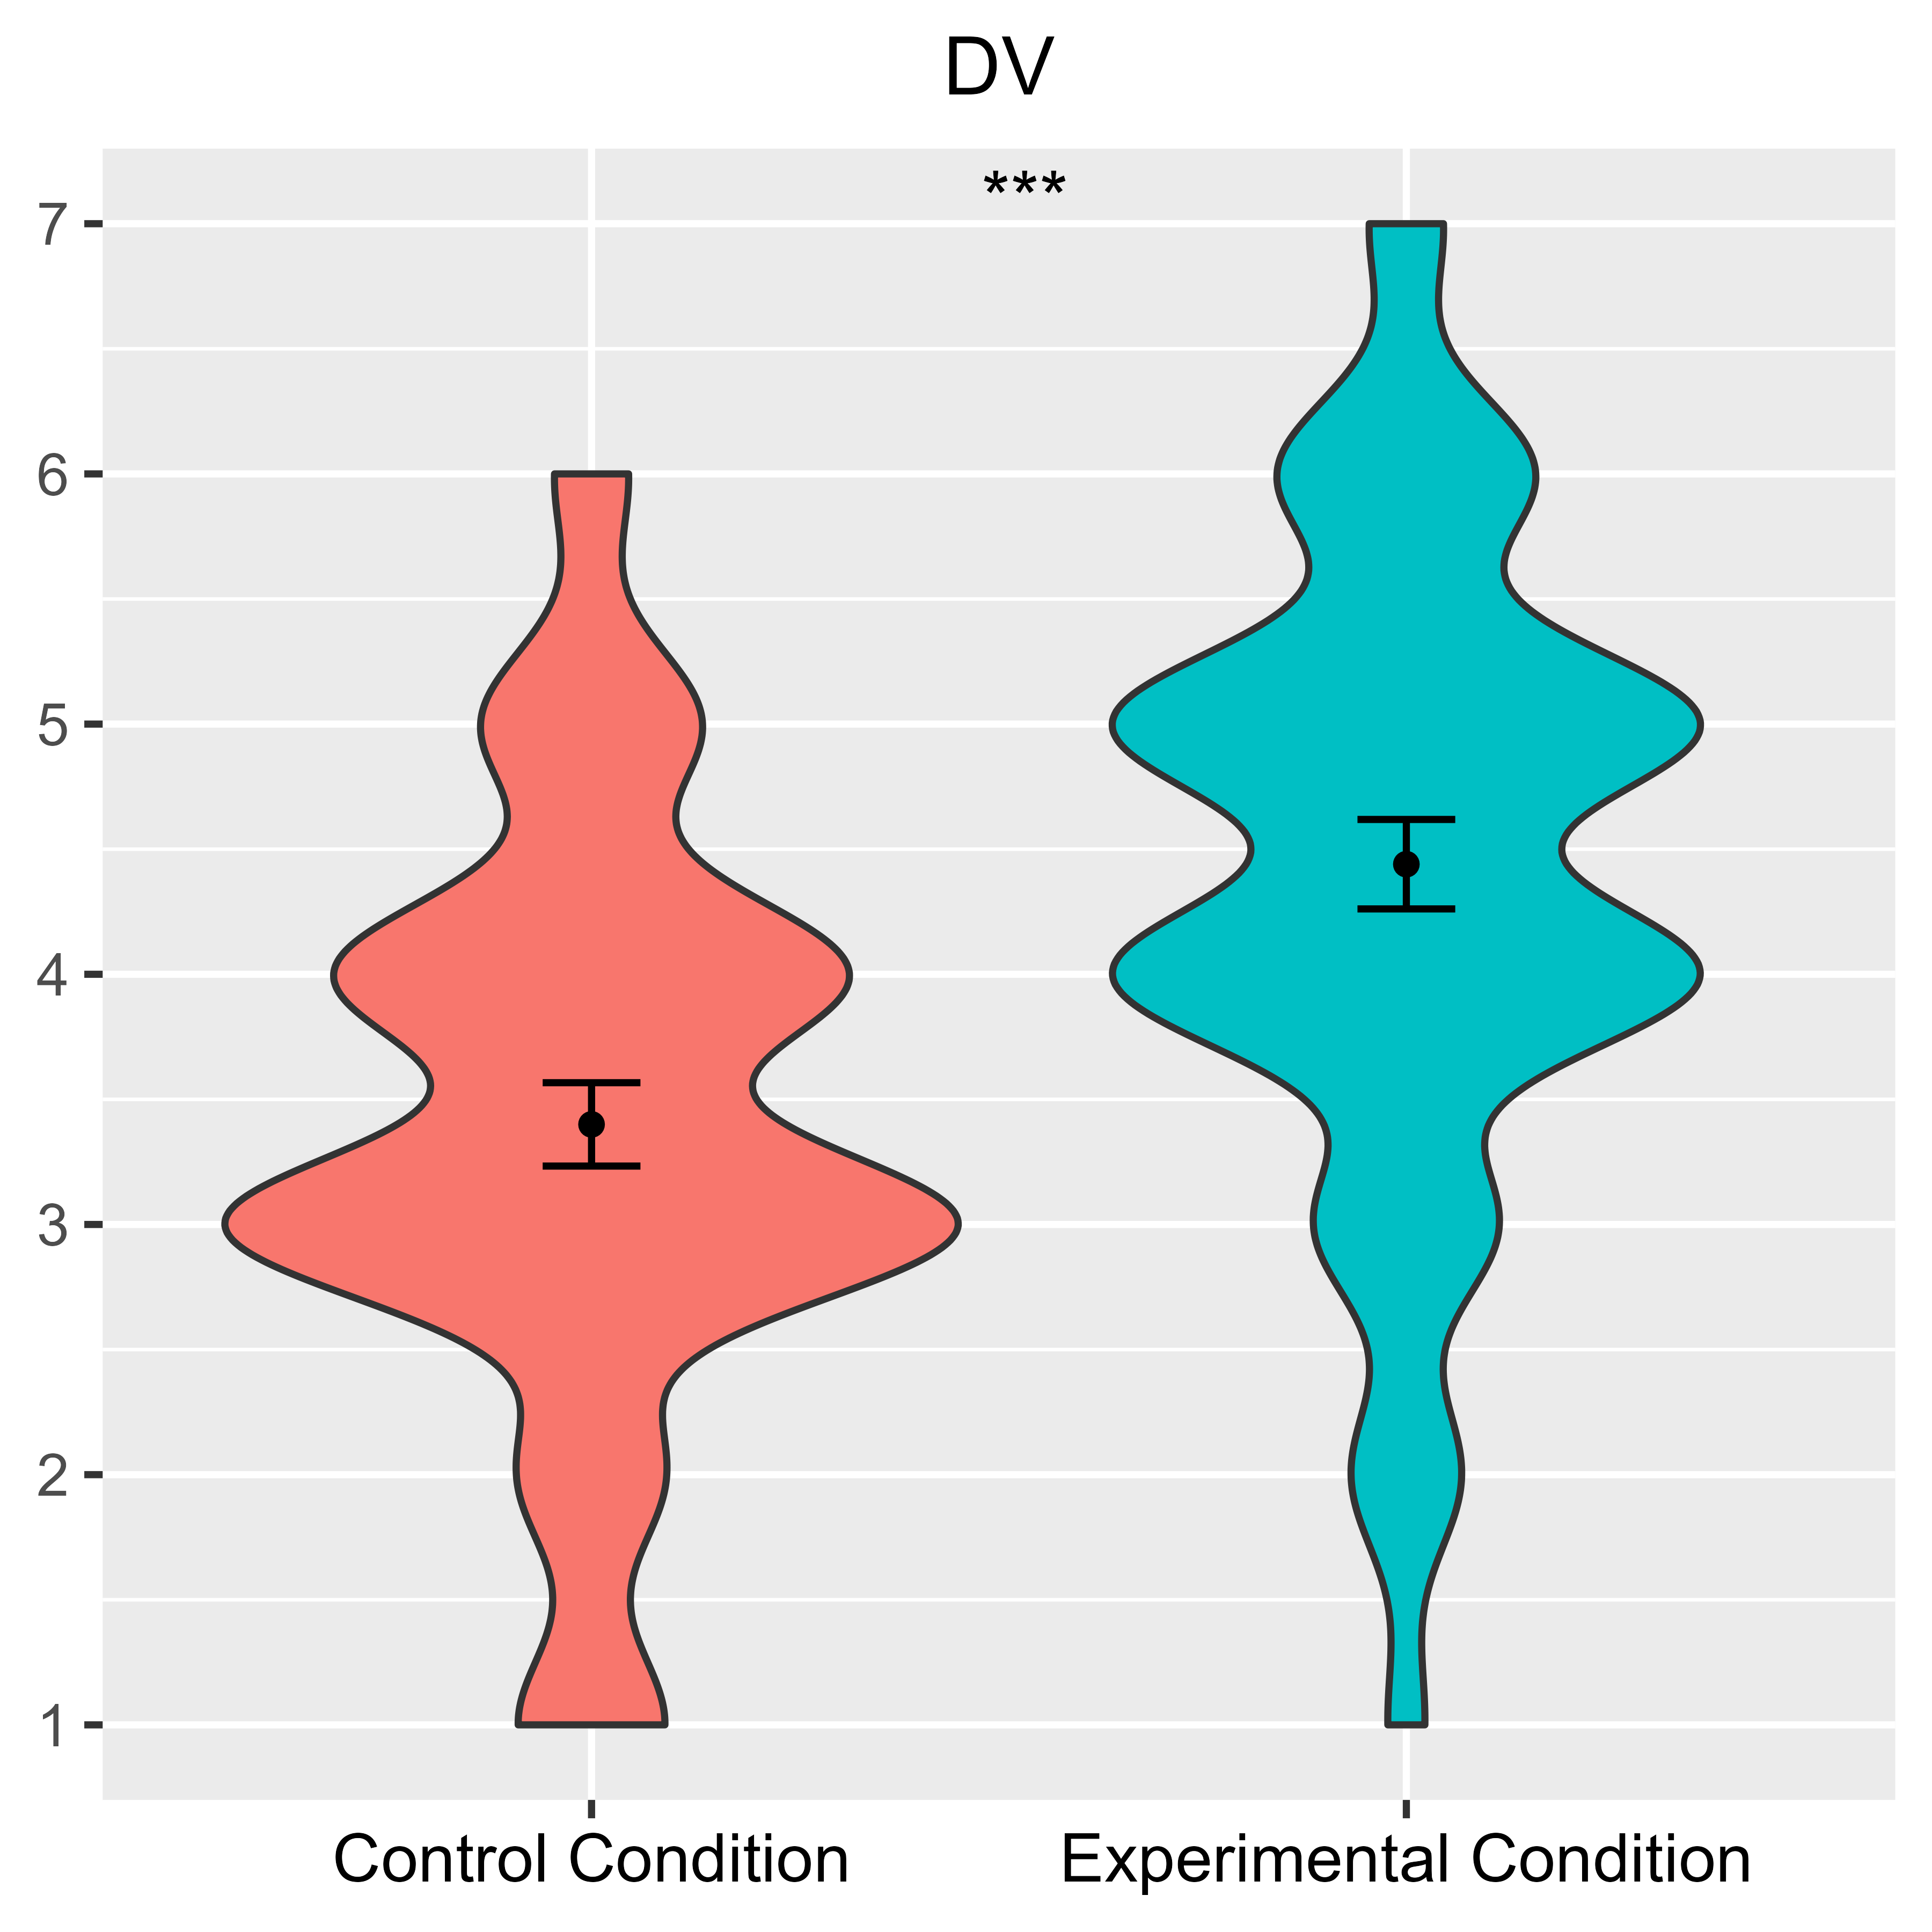
\includegraphics[width=\linewidth,height=0.3\textheight]{images/Study 1/DV 1.png}
    \end{subfigure}
    \hfill
    \begin{subfigure}{0.48\linewidth}
        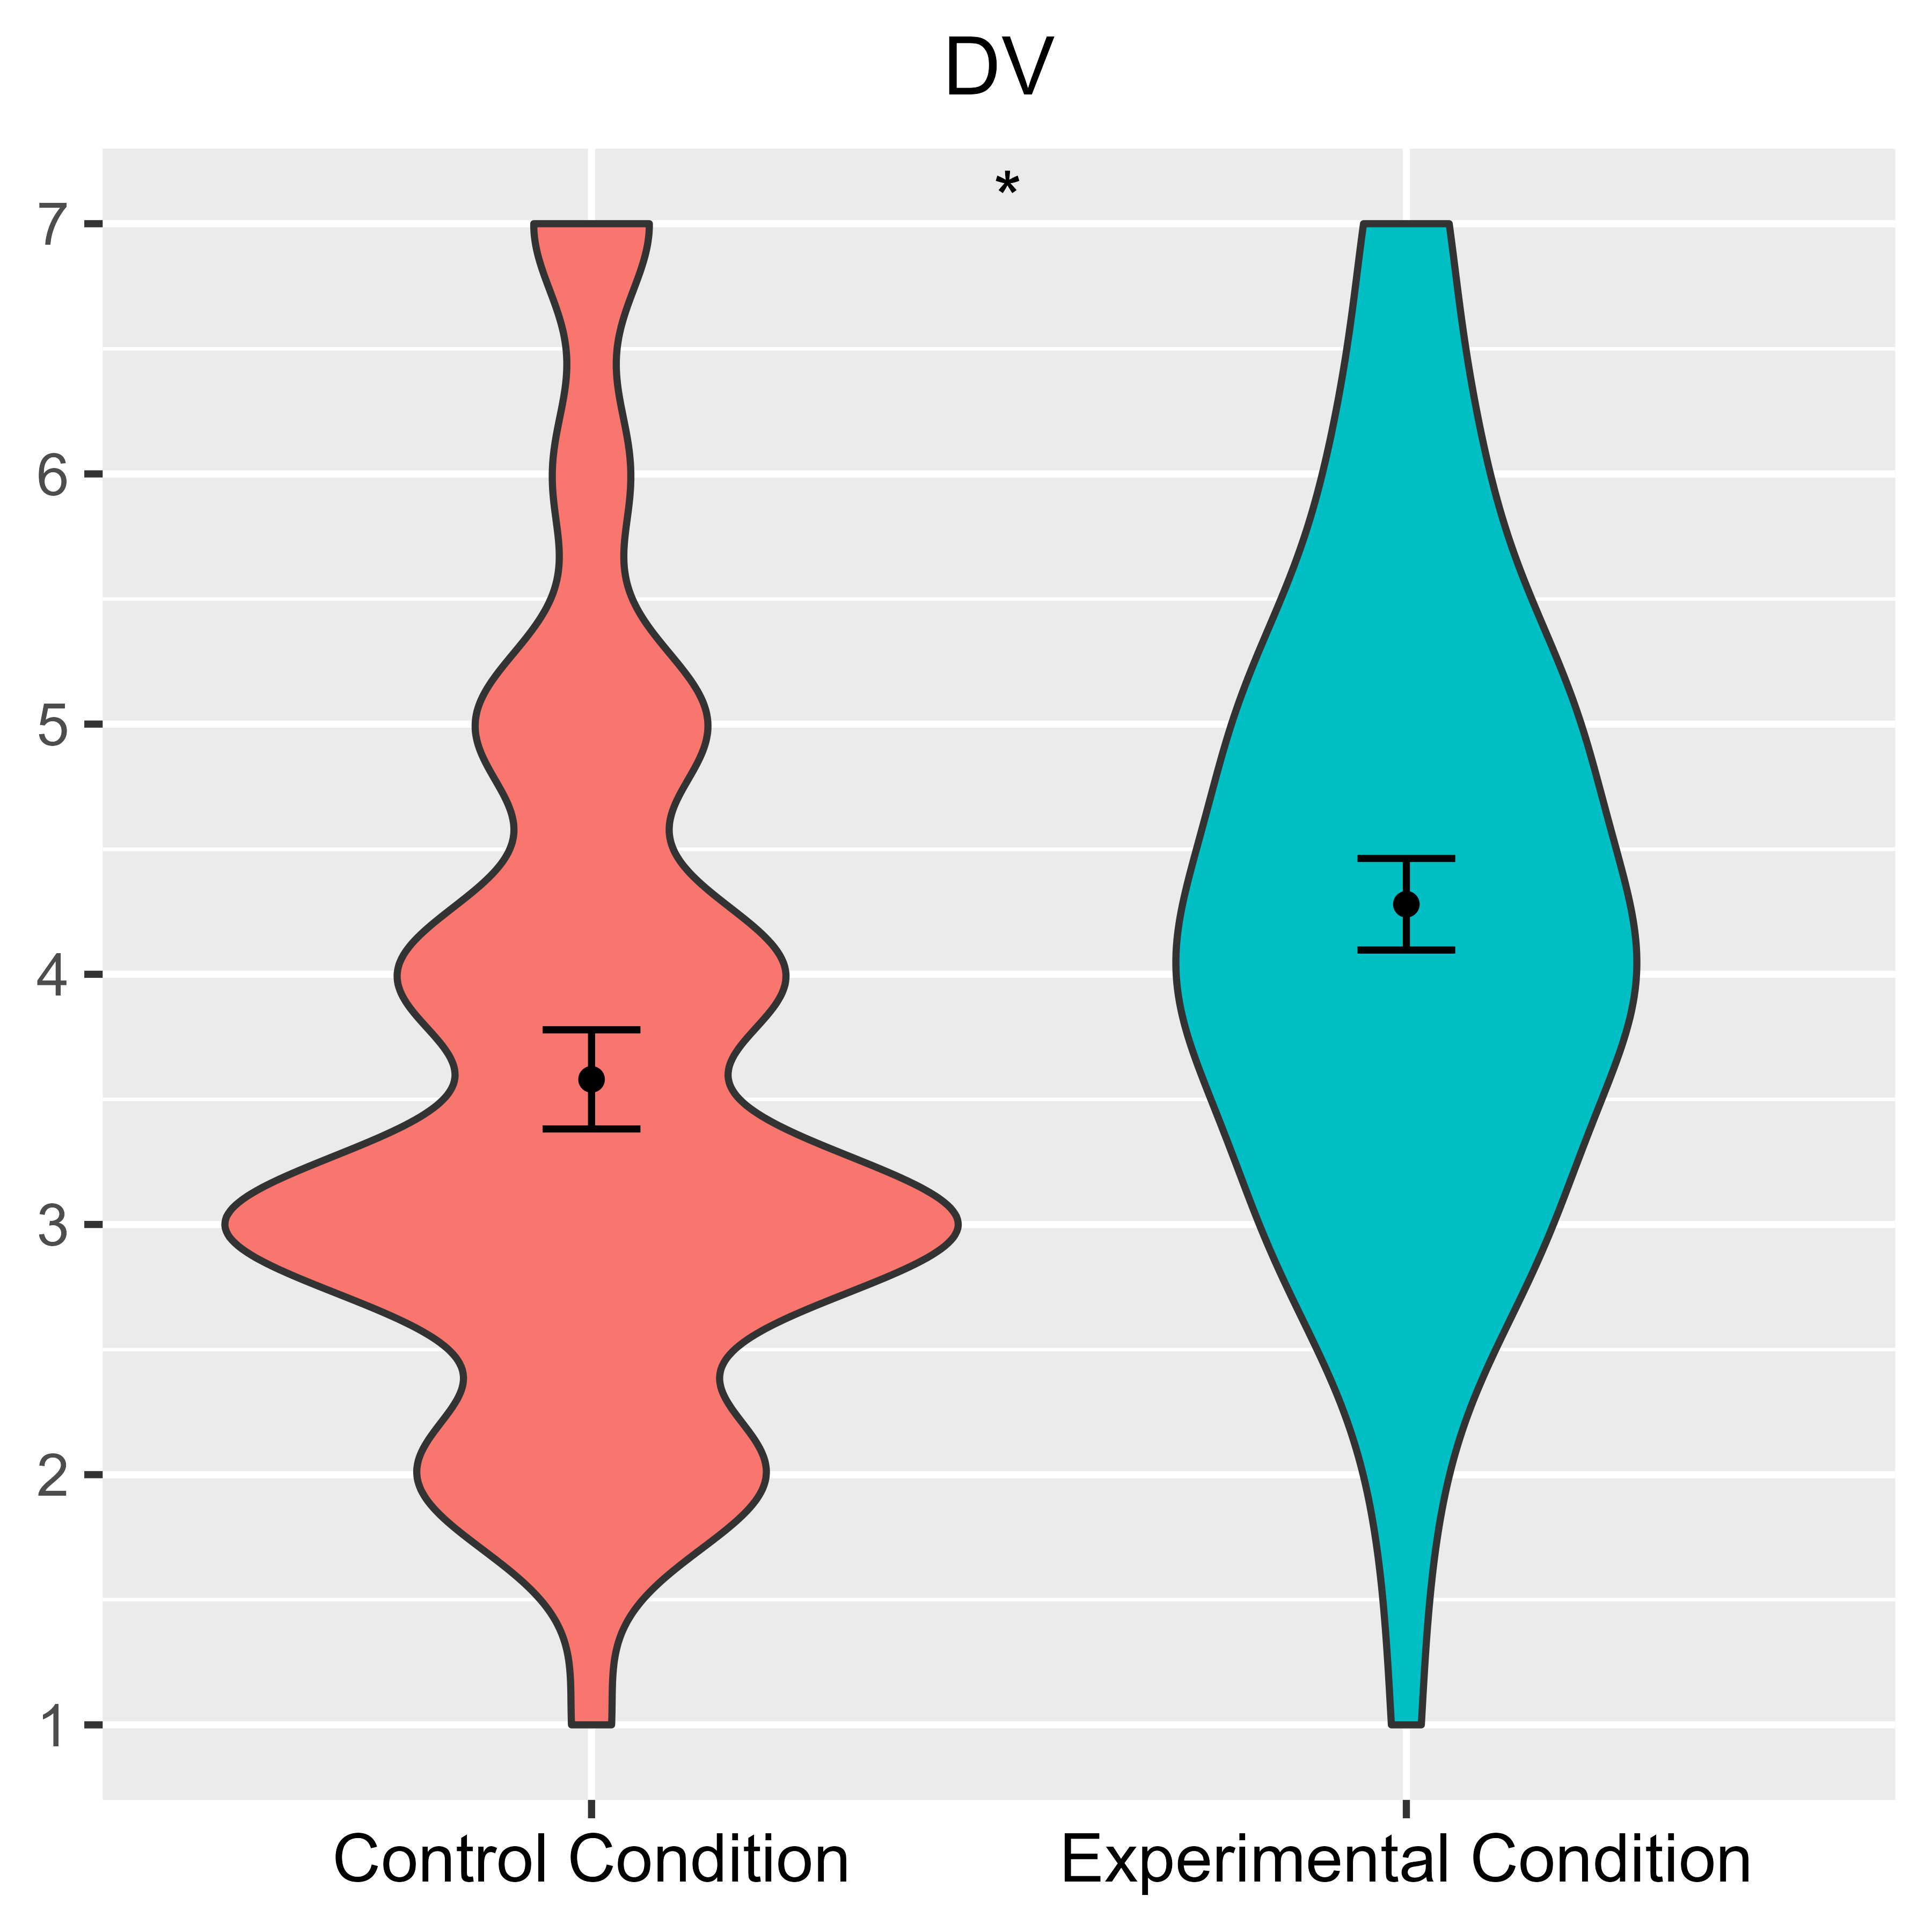
\includegraphics[width=\linewidth,height=0.3\textheight]{images/Study 1/DV 2.png}
    \end{subfigure}

    \captionsetup{justification=justified, labelfont=bf, font=footnotesize, singlelinecheck = false, labelsep=period}
    \caption[Figure Name Shown on the List of Figures]{Caption and footnotes of figure 1 (fake data)}
    \label{fig: Study 1, DV1-2}
\end{figure}

independent sample t-tests found ... (see Fig. \ref{fig: Study 1, DV1-2}). 

\subsection{Discussion}

brief discussion
\section{Study 2}

\subsection{Methods}

\subsubsection{Participants}

sample size, demographics, participant fees, informed consent

\subsubsection{Design \& Materials}

procedures, IVs, DVs, etc.

\subsection{Results}

\begin{table}[ht]
\centering
\fontsize{10pt}{12pt}\selectfont
\caption{Example Table (Fake)}
\begin{tabular}{llllll}
    \toprule
    DV& \textit{M}& 95\%\textit{CI} &   $df$&\textit{t}&\textit{p} \\
    \midrule
    DV1 & 1.23 & [0.99, 1.99] & 99 & 1.98 & .003 \\
    DV2 & 2.34 & [1.99, 2.99] & 99 & 2.76 & .002 \\
    DV3 & 3.56 & [2.99, 3.99] & 99 & 3.54 & .001 \\
    \bottomrule
\end{tabular}
\label{tab: Study 2 Example Table}
\end{table}

One sample t-tests revealed ... (see Table \ref{tab: Study 2 Example Table})

\subsection{Discussion}

brief discussion
\include{docs/5-General Discussion}
\include{docs/6-Conclusion}

% References
\printbibliography[heading=bibnumbered]

% Re-count tables and figures
\setcounter{table}{0}
\setcounter{figure}{0}
% Add "S" before the number e.g., Table S1, Figure S1
\renewcommand{\thetable}{S\arabic{table}}
\renewcommand{\thefigure}{S\arabic{figure}}

% include appendix
%TC:ignore

\section{Appendix - Supplementary Results}
\label{Appendix B}

\subsection*{Study 1}

\begin{longtable}{p{0.4\textwidth} p{0.3\textwidth} p{0.2\textwidth}}

\toprule
Demographics & Final Sample (\textit{N} = 100) & All (\textit{N} = 200)\\
\midrule
\endfirsthead

\toprule
Demographics & Final Sample (\textit{N} = 100) & All (\textit{N} = 200)\\
\midrule
\endhead

\textbf{Age range (\%)} & \\
18-24 years old & 10 (10\%) & 20 (10\%) \\
25-34 years old & 10 (10\%) & 20 (10\%) \\
35-44 years old & 20 (20\%) & 40 (20\%) \\
45-54 years old & 30 (30\%) & 60 (30\%) \\
55-64 years old & 30 (30\%) & 60 (30\%) \\
65 years or older & 0 (0\%) & 0 (0\%) \\

\textbf{Gender (\%)} & \\
Male & 40 (40\%) & 80 (40\%) \\
Female & 50 (50\%) & 100 (50\%) \\
Other & 5 (5\%) & 10 (5\%) \\
Prefer not to say & 5 (5\%) & 10 (5\%) \\

\textbf{Education (\%)} & \\ 
No schooling completed & 0 (0\%) & 0 (0\%) \\
High school graduates, diploma or equivalent & 20 (20\%) & 40 (20\%) \\
Some college, no degree & 30 (30\%) & 60 (30\%) \\
Bachelor's degree & 40 (40\%)  & 80 (40\%) \\
Graduate degree & 10 (10\%) & 20 (10\%) \\
Prefer not to say & 0 (0\%) & 0 (0\%) \\

\textbf{Ethnic origin (\%)} & \\
Asian & 30 (30\%) & 30 (30\%) \\
Black or African & 30 (30\%) & 60 (30\%) \\
White or Caucasian & 30 (30\%) & 60 (30\%) \\
Other & 5 (5\%) & 10 (5\%) \\
Prefer not to say & 5 (5\%) & 10 (5\%)\\

\textbf{Conditions (\%)} \\
Control Condition & 50 (50\%) & 100 (50\%) \\
Experimental Condition & 50 (12.3\%) & 100 (50\%) \\
\bottomrule

\captionsetup{justification=raggedright, labelfont=bf, singlelinecheck = false, labelsep=period}
\caption{Demographic information of participants in Study 1 (Fake).}
\label{tab: Study 1 Demographics}
\end{longtable}

%TC:endignore

\end{document}